\documentclass[journal]{IEEEtran}

\usepackage{amsmath}
\usepackage{cite}
\usepackage{hyperref}
\usepackage{graphicx}
\usepackage{caption}
\usepackage{array}
\usepackage{url}
% \usepackage[spanish]{babel}
\def\UrlBreaks{\do\/\do-}
% *** GRAPHICS RELATED PACKAGES ***
%
\ifCLASSINFOpdf
  % \usepackage[pdftex]{graphicx}
  % declare the path(s) where your graphic files are
  % \graphicspath{{../pdf/}{../jpeg/}}
  % and their extensions so you won't have to specify these with
  % every instance of \includegraphics
  % \DeclareGraphicsExtensions{.pdf,.jpeg,.png}
\else
\fi



\begin{document}


\title{Comparación de técnicas basadas en datos para la predicción de potencia en una turbina a partir de datos meteorológicos de una estación cercana}

\author{Diego Lera, Antonio Martínez-Gandía}% <-this % stops a space

\markboth{IEEE TRANSACTIONS ON NEURAL NETWORKS AND LEARNING SYSTEMS, VOL. 32, NO. 5, APRIL 2020}%
{Shell \MakeLowercase{\textit{et al.}}: Bare Demo of IEEEtran.cls for IEEE Journals}

\maketitle

% As a general rule, do not put math, special symbols or citations
% in the abstract or keywords.
\begin{abstract}
Se han realizado muchos estudios para la predicción tanto meteorológica, como de potencia en fuentes de energía renovable. En estos se hace una clara distinción entre métodos numéricos, que se basan en crear modelos utilizando ecuaciones de la física, y métodos estadísitos o de aprendizaje. En este documento pretendemos comparar la eficacia de cuatro técnicas de \emph{machine learning}, tanto en predicción de potencia como en predicción de viento.
Los métodos utilizados son: regresión lineal, KNN, MARS y redes LSTM. Con estos cuatro métodos tenemos algoritmos de muy distinta complejidad utilizados en dos aplicaciones también muy distintas.

Para unir los dos casos de uso se plantea la predicción de la potencia generada por una turbina y del viento en su ubicación, partiendo de los datos de una estación meteorológica situada a 15 km, en la provincia de Yalova, Turquía.

La distancia entre la turbina y la estación, junto con el ruido y las imperfecciones de los \emph{datasets} utilizados, presentan grandes problemas para los modelos. Sin embargo, los resultados obtenidos con MARS y KNN podrían ser válidos para realizar una aplicación encadenada entre las dos predicciones, para conseguir valores de potencia en la turbina a partir de la predicción meteorológica del día siguiente.
\end{abstract}

% Note that keywords are not normally used for peerreview papers.
\begin{IEEEkeywords}
KNN, MARS, LSTM, Regresion, I+D+i, machine learning, wind forecasting.
\end{IEEEkeywords}






\IEEEpeerreviewmaketitle



\section{Introducción}
\IEEEPARstart{S}{i} queremos predecir la potencia generada por una planta de energía renovable necesitamos conocer las condiciones meteorológicas en los próximos días. Esta información sólo suele recopilarse en las estaciones meteorológicas, y éstas pueden encontrarse lejos de la planta. 

Como solución a este problema planteamos el uso de cuatro técnicas de \emph{machine learning}: Regresión Lineal, Regresión por K-vecinos (KNN), MARS y redes LSTM, que compararemos para descubrir cúal presenta mejores resultados.

El problema en concreto se centra en  predecir la potencia de una turbina eólica situada en la provincia de Yalova, Turquía ( X:668478 Y:4494833 UTM ED 50, 6 degree), cuya estación meteorológica más cercana se encuentra en la capital, a 15 kilómetros de las turbinas.
Para el entrenamiento de los algoritmos utilizaremos dos bases de datos. Una con la relación entre la potencia generada por la turbina y las características del viento (velocidad y dirección) en su ubicación, y otra con los datos meteorológicos de la estación.


Ante el problema de la predicción meteorológica existen dos enfoques principales: el uso de modelos numéricos con ecuaciones extraídas de la física y modelos estadísticos, principalmente utilizando técnicas de \emph{machine learninrg}. \cite{FOLEY20121} En general, los métodos numéricos consiguen buenos resultados calculando medias mensuales o anuales de variables macroscópicas como la temperatura o presión, mientras que los estadísticos consiguen buenas predicciones a corto plazo, día por día u hora por hora. \cite{FOLEY20121} \cite{GIEBEL2003}.
Existen múltiples estudios destinados a la predicción meteorológica con técnicas de \emph{machine learning}, concretando para nuestro problema, el artículo de Xingjian Shi, Zhourong Chen, Hao Wang y Dit-Yan Yeung  para la predicción de precipitaciones usando redes LSTM\cite{NIPS2015_5955}, que arroja buenos resultados con una correlación de hasta un 0.908. Un estudio de la predicción de la irradiancia de un año entero realizado por Xiangyun Qing y Yugang Niu muestra mejoras respecto a otra red convolucional como BPNN \cite{QING2018461}.

Por ser el método más común de aprendizaje automático utilizaremos también técnicas de regresión, tanto lineal, como por K-vecinos como por splines (MARS). El método por K-vecinos ha presentado buenos resultados en el campo de la predicción meteorológica por su robustez en distribuciones irregulares \cite{HUANG201789}. Las técnicas de regresión con splines multivariantes adaptativos (MARS) también han sido escogidos en distintos experimentos relaccionados con la predicción de variables ambientales a corto plazo por su robustez, al no depender de presuposiciones acerca del comportamiento y su capacidad para aproximar modelos no lineales \cite{KRZEMIEN2019777} \cite{PA_LEWIS1991_864}.


A continuación, se explican brevemente las bases de cada una de las técnicas que realizamos en este artículo:
\begin{itemize}
    \item Regresión Lineal: Se trata de un método matemático para aproximar la relación entre una variable $Y$ y unas variables independientes $X_i$, ajustando unos parámetros $a_i$, de la forma:
\begin{equation}
\label{eqn:Reg}
 Y = a_0+a_1X_1 + a_2X_2+\ldots + a_nX_n
\end{equation}

    \item Regresión KNN: A diferencia del anterior, este es un método no paramétrico. Permite aproximar funciones no lineales y muy variantes \cite{James2013}. Dado un conjunto de datos de entrenamiento, se calcula la salida de un nuevo dato como la media de las salidas de los K valores más cercanos (vecinos) en el conjunto de entrenamiento.
    \item MARS: Se trata de un procedimiento adaptativo de regresión. Basado en unas funciones básicas llamadas \emph{splines}, que siguen las siguientes ecuaciones: 
    \begin{figure}[!ht]
        \centering
        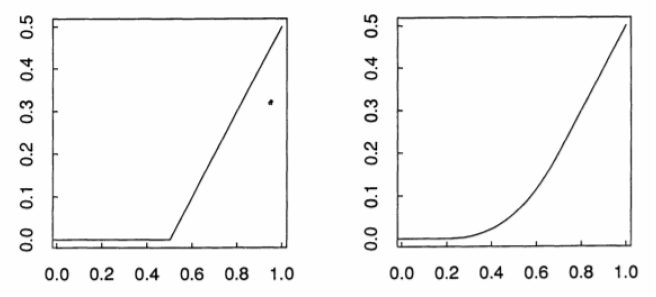
\includegraphics[width=6cm, height=2.5cm]{Splines.png}
        \captionsetup{justification=centering,singlelinecheck=false}
        \caption{Ejemplo de spline lineal y spline cúbico}
        \label{fig:splines}
    \end{figure}
    El método consiste en encontrar una combinación de estos splines que aproxime mejor el comportamiento de los datos de entrada para generar un modelo que nos permita hacer una predicción. Segun Friedman, \cite{JHFRIEDMAN1991} el método consigue mejores resultados que el KNN en problemas con altas dimensiones.
    \item LSTM: Son redes neuronales recurrentes (RNN). Se pueden aproximar como una cadena de redes neuronales en la que cada una pasa un mensaje a su sucesora. Son muy utilizadas para tratar datos secuenciales de mayor tamaño que las RNN tradicionales, muy utilizadas en reconocimiento de habla o de imágenes. La capacidad para tratar grandes cadenas de datos se consigue gracias a la eliminación del problema de desvanecimiento de gradiente al ajustar los parámetros de las neuronas durante el \emph{backpropagation} \cite{45500}.

\end{itemize}


\section{Métodos}
Para afrontar el problema lo dividimos en dos partes. En primer lugar, nos centramos en la predicción de la potencia con los datos del viento en la ubicación de la turbina. En segundo lugar, calcularemos el viento en dicha ubicación a partir de los datos de la estación meteorológica de Yalova. 

Los datos han de estar tomados en los mismos instantes de tiempo. El \emph{dataset} de la potencia de la turbina nos ofrece los datos tomados cada diez minutos, comenzando el 01/01/2018 y terminando el 31/12/2018.  Por otro lado, la estación meteo-rológica nos ofrece un histórico de los datos del mismo año con una periodicidad de 3 horas, por lo que, para la predicción de viento, debemos eliminar los datos no coincidentes.  


Los \emph{datasets} utilizados se han extraido de las páginas kaggle.com y worldweatheronline.com respectivamente. Se pueden encontrar adaptados en el siguiente repositorio: \url{https://github.com/DiegoLera/TurbinaYalova}

Todos los métodos explicados en este documento se han llevado a cabo con MATLAB, en la versión R2019a.

Para realizar una limpieza de los datos de la turbina, se realiza una eliminación de los que correspondan a: paradas de la turbina ($P=0$) y momentos en los que la potencia teórica y real difieren en exceso ($P_{teorica}>P_{real}+500$).
Posteriormente, se ha hecho una división de los datos para las fases de entrenamiento, validación y test, de forma aleatoria sobre cada base de datos y con una proporción del 70\%, 20\% y 10\%, respectivamente. Para las redes LSTM no podemos escoger aleatoriamente los datos para no romper la secuencialidad. El método utilizado se explica más adelante.

Obtención de los modelos:

\begin{itemize}
    \item Regresión Lineal: Para obtener el grado del polinomio indicado en la ecuación \ref{eqn:Reg} se realiza un proceso iterativo en el que en cada paso se aumenta un grado el orden del polinomio y se calcula el MSE, escogiéndose el grado en el que se presente un mínimo. 
    \item Regresión KNN: Se calculan los valores de salida para los datos de validación utilizando como entradas los datos de entrenamiento. Realizamos el proceso con valores de K de 1 a 100 y seleccionamos el que menor valor MSE proporcione para los datos de validación.
    \item MARS: Utilizamos la toolbox de MATLAB llamada ARESLab, que integra todas las funciones explicadas por Friedman en su artículo sobre el método \cite{JHFRIEDMAN1991}. En primer lugar, definimos los parámetros del proceso con la función \emph{aresparams2}, tal como se indica en la documentación de la toolbox \cite{ARESLAB2016}. Definimos:
    \begin{itemize}
        \item $maxFuncs = 20$ ($30$ en la predicción de viento)
        \item $maxIterations = 1$ ($3$ en la predicción de viento)
        \item $useMinSpan = 2$
        \item $useEndSpan = 2$
    \end{itemize}
    En el modelo de la predicción de viento aumentamos el número de funciones máximo y de iteraciones, ya que se utilizan muchas más entradas y el algoritmo requiere más flexibilidad.
    Para construir el modelo se utiliza la función \emph{aresbuild}, a la que aportamos los datos de entrenamiento y validación juntos, ya que internamente ya se realiza la fase de validación.
    Para calcular el error del modelo utilizamos la función \emph{arestest} con los datos de test.
    \item LSTM: Dada la importancia de la secuencialidad de los datos, no se pueden seleccionar particiones aleatorias para el entrenamiento de la red.  Para la preparación de los datos de entrenamiento hemos realizado un proceso iterativo en el que se realizan particiones manteniendo la secuencialidad. Comenzamos dividiendo los datos de entrenamiento creando un conjunto cada día y calculando el error de la red. En cada paso se aumenta en un día los conjuntos de datos, es decir, en el segundo paso se dividen los conjuntos cada dos días, y así sucesivamente hasta llegar a la última iteración, en la que se crea un conjunto único con todos los datos en un conjunto.
    Para la creación de la red se utiliza la \emph{toolbox} de Matlab para la creación de redes neuronales. Se especifícan las características de la red mediante los parámetros contenidos en el \emph{array layer}.

\end{itemize}

% An example of a floating figure using the graphicx package.
% Note that \label must occur AFTER (or within) \caption.
% For figures, \caption should occur after the \includegraphics.
% Note that IEEEtran v1.7 and later has special internal code that
% is designed to preserve the operation of \label within \caption
% even when the captionsoff option is in effect. However, because
% of issues like this, it may be the safest practice to put all your
% \label just after \caption rather than within \caption{}.
%
% Reminder: the "draftcls" or "draftclsnofoot", not "draft", class
% option should be used if it is desired that the figures are to be
% displayed while in draft mode.
%
%\begin{figure}[!t]
%\centering
%\includegraphics[width=2.5in]{myfigure}
% where an .eps filename suffix will be assumed under latex, 
% and a .pdf suffix will be assumed for pdflatex; or what has been declared
% via \DeclareGraphicsExtensions.
%\caption{Simulation results for the network.}
%\label{fig_sim}
%\end{figure}

% Note that the IEEE typically puts floats only at the top, even when this
% results in a large percentage of a column being occupied by floats.
\section{Resultados} 
Tras realizar los modelos se han evaluado los resultados utilizando la partición de datos de test. Los errores cometidos en las predicciones para cada método se pueden ver en la Tabla~\ref{t:resRMSE}, expresados en la raíz del error cuadrático medio (RMSE).

Para la regresión lineal el mínimo en el error se presenta para un orden 7, por lo que el polinomio del modelo es del mismo orden.

Para el KNN, los valores óptimos de $K$ son $38$, en la predicción de potencia, y $7$ para la predicción de viento.

Tras realizar los cálculos con MARS obtenemos unos modelos construidos con 9 funciones básicas (splines), 17 parámetros  y 2 variables de entrada para el modelo de predicción de potencia, y 14 funciones básicas, 27 parámetros y 7 variables de entrada para el modelo de predicción de viento.

La iteración para el conjunto de datos de la LSTM explicado anteriormente, presenta un error mínimo al realizar una agrupación de los datos cada 3 días.
% \begin{table}[ht]
% \centering
% \caption{Resultados en MSE}\label{t:res}
% \begin{tabular}{|l|c|c|}
% \hline
% & Predicción de viento (MSE) & Predicción de potencia (MSE)\\ \hline
% Regresión lineal & 67 & 12811 \\ \hline
% KNN & 9.6739 & 9223 \\ \hline
% MARS & 11.59 & 10840 \\ \hline
% LSTM & 17.62 & 163500 \\ \hline
% \end{tabular}
% \end{table}

\begin{table}[h]
% \centering
\caption{Resultados en RMSE}\label{t:resRMSE}
\begin{tabular}{|>{\centering}p{0.125\textwidth}| >{\centering}p{0.125\textwidth} | >{\centering\arraybackslash}p{0.125\textwidth}|}

\hline
&Predicción de viento (RMSE) & Predicción de potencia (RMSE)\\ \hline
Regresión lineal & 8.18 & 113.19 \\ \hline
KNN & 3.18 & 93.8 \\ \hline
MARS & 3.30 & 101.07 \\ \hline
LSTM & 4.20 & 404.35 \\ \hline
\end{tabular}
\end{table}

% An example of a double column floating figure using two subfigures.
% (The subfig.sty package must be loaded for this to work.)
% The subfigure \label commands are set within each subfloat command,
% and the \label for the overall figure must come after \caption.
% \hfil is used as a separator to get equal spacing.
% Watch out that the combined width of all the subfigures on a 
% line do not exceed the text width or a line break will occur.
%
%\begin{figure*}[!t]
%\centering
%\subfloat[Case I]{\includegraphics[width=2.5in]{box}%
%\label{fig_first_case}}
%\hfil
%\subfloat[Case II]{\includegraphics[width=2.5in]{box}%
%\label{fig_second_case}}
%\caption{Simulation results for the network.}
%\label{fig_sim}
%\end{figure*}
%
% Note that often IEEE papers with subfigures do not employ subfigure
% captions (using the optional argument to \subfloat[]), but instead will
% reference/describe all of them (a), (b), etc., within the main caption.
% Be aware that for subfig.sty to generate the (a), (b), etc., subfigure
% labels, the optional argument to \subfloat must be present. If a
% subcaption is not desired, just leave its contents blank,
% e.g., \subfloat[].


% An example of a floating table. Note that, for IEEE style tables, the
% \caption command should come BEFORE the table and, given that table
% captions serve much like titles, are usually capitalized except for words
% such as a, an, and, as, at, but, by, for, in, nor, of, on, or, the, to
% and up, which are usually not capitalized unless they are the first or
% last word of the caption. Table text will default to \footnotesize as
% the IEEE normally uses this smaller font for tables.
% The \label must come after \caption as always.
%
%\begin{table}[!t]
%% increase table row spacing, adjust to taste
%\renewcommand{\arraystretch}{1.3}
% if using array.sty, it might be a good idea to tweak the value of
% \extrarowheight as needed to properly center the text within the cells
%\caption{An Example of a Table}
%\label{table_example}
%\centering
%% Some packages, such as MDW tools, offer better commands for making tables
%% than the plain LaTeX2e tabular which is used here.
%\begin{tabular}{|c||c|}
%\hline
%One & Two\\
%\hline
%Three & Four\\
%\hline
%\end{tabular}
%\end{table}

\section{Discusión}
Para cuantificar los resultados necesitaríamos comparar con otros experimentos realizados en condiciones similares, de los que no disponemos. Este estudio queda como referencia para posibles ampliaciones y comparación con otros trabajos.

Por otro lado, tras observar los resultados, se aprecia que la ruptura de la continuidad en los \emph{datasets} ha influido en la técnica LSTM, en la que la secuencialidad es una parte fundamental para su entrenamiento. 

Con respecto a las otras técnicas, las tres consiguen resultados muy similares, con la excepción de la regresión lineal en la predicción de viento, que presenta un error  un 157.23\% mayor que el KNN, que es el que mejores resultados obtiene en ambos casos. 


Una posible ampliación de este proyecto consiste en el análisis del \emph{dataset} de entrada para la predicción del viento seleccionando las variables con mayor relevancia mediante la matriz de correlación.

Por último, si se desea aplicar esto a una predicción real, bastaría con utilizar como entrada una predicción meteorológica y encadenar los dos modelos con menor error (KNN en ambos casos) para obtener una salida de potencia.

\section{Conclusión}
Las técnicas estadísticas dependen mucho de la calidad de los datos con los que se trabaje. Cuando no se dispone de una calidad adecuada, las técnicas que no dependen de la linealidad o secuencialidad de los datos son más eficaces.






% if have a single appendix:
%\appendix[Proof of the Zonklar Equations]
% or
%\appendix  % for no appendix heading
% do not use \section anymore after \appendix, only \section*
% is possibly needed

% use appendices with more than one appendix
% then use \section to start each appendix
% you must declare a \section before using any
% \subsection or using \label (\appendices by itself
% starts a section numbered zero.)
%




% you can choose not to have a title for an appendix
% if you want by leaving the argument blank


% use section* for acknowledgment

\medskip

\bibliographystyle{IEEEtran}
\bibliography{Bibliografia}


% Can use something like this to put references on a page
% by themselves when using endfloat and the captionsoff option.
\ifCLASSOPTIONcaptionsoff
  \newpage
\fi



% trigger a \newpage just before the given reference
% number - used to balance the columns on the last page
% adjust value as needed - may need to be readjusted if
% the document is modified later
%\IEEEtriggeratref{8}
% The "triggered" command can be changed if desired:
%\IEEEtriggercmd{\enlargethispage{-5in}}

% references section

% can use a bibliography generated by BibTeX as a .bbl file
% BibTeX documentation can be easily obtained at:
% http://mirror.ctan.org/biblio/bibtex/contrib/doc/
% The IEEEtran BibTeX style support page is at:
% http://www.michaelshell.org/tex/ieeetran/bibtex/
%\bibliographystyle{IEEEtran}
% argument is your BibTeX string definitions and bibliography database(s)
%\bibliography{IEEEabrv,../bib/paper}
%
% <OR> manually copy in the resultant .bbl file
% set second argument of \begin to the number of references
% (used to reserve space for the reference number labels box)
% \begin{thebibliography}{1}

% \bibitem{IEEEhowto:kopka}
% H.~Kopka and P.~W. Daly, \emph{A Guide to \LaTeX}, 3rd~ed.\hskip 1em plus
%   0.5em minus 0.4em\relax Harlow, England: Addison-Wesley, 1999.

% \bibliography{convolutional-lstm-network-a-machine-learning-approach-for-precipitation-nowcasting}{}       % expects file "myrefs.bib"

% \end{thebibliography}

% biography section
% 
% If you have an EPS/PDF photo (graphicx package needed) extra braces are
% needed around the contents of the optional argument to biography to prevent
% the LaTeX parser from getting confused when it sees the complicated
% \includegraphics command within an optional argument. (You could create
% your own custom macro containing the \includegraphics command to make things
% simpler here.)
%\begin{IEEEbiography}[{\includegraphics[width=1in,height=1.25in,clip,keepaspectratio]{mshell}}]{Michael Shell}
% or if you just want to reserve a space for a photo:


% You can push biographies down or up by placing
% a \vfill before or after them. The appropriate
% use of \vfill depends on what kind of text is
% on the last page and whether or not the columns
% are being equalized.

%\vfill

% Can be used to pull up biographies so that the bottom of the last one
% is flush with the other column.
%\enlargethispage{-5in}



% that's all folks
\end{document}
